%==============================================================
%  PREAMBLE — RVCC MAT-251 Master Document Noah Berns
%==============================================================

\documentclass[9pt]{amsart}

%--------------------------------------------------------------
%  Encoding & Language
%--------------------------------------------------------------
\usepackage[utf8]{inputenc}
\usepackage[english]{babel}

%--------------------------------------------------------------
%  Mathematics
%  (load amsmath/mathtools BEFORE amsthm)
%--------------------------------------------------------------
\usepackage{amssymb}
\usepackage{mathtools}      % pulls in amsmath automatically
\usepackage{amsthm}

%--------------------------------------------------------------
%  Graphics, Floats & Captions
%--------------------------------------------------------------
\usepackage{graphicx}       % images
\usepackage{float}          % [H] float placement
\usepackage{wrapfig}        % wrapped figures
\usepackage{caption}
\usepackage{subcaption}     % subfigures (also loads caption)
\usepackage{pdfpages}       % include external PDFs

%--------------------------------------------------------------
%  Tables, Lists & Color
%--------------------------------------------------------------
\usepackage{tabularx}
\usepackage{enumitem}
\usepackage{xcolor}

%--------------------------------------------------------------
%  Plotting
%--------------------------------------------------------------
\usepackage{pgfplots}
\pgfplotsset{compat=newest}

%--------------------------------------------------------------
%  Boxes, Spacing & Misc
%--------------------------------------------------------------
\usepackage{tcolorbox}
\usepackage{setspace}
\usepackage{textcomp}
\usepackage[symbol]{footmisc}
\usepackage{blindtext}      % dummy text — remove for the final version

%--------------------------------------------------------------
%  Page Geometry
%--------------------------------------------------------------
\usepackage[a4paper, total={6in, 8in}]{geometry}

%--------------------------------------------------------------
%  Hyperlinks  (load after most packages; biblatex goes after it)
%--------------------------------------------------------------
\usepackage{url}            % redundant with hyperref, but harmless
\usepackage{hyperref}

%--------------------------------------------------------------
%  Bibliography  (biblatex + biber)
%  Put \printbibliography in the BODY where the references go.
%--------------------------------------------------------------
\usepackage[autostyle]{csquotes}            % must precede biblatex
\usepackage[backend=biber, sorting=none]{biblatex}
\addbibresource{MyBib.bib}

%==============================================================
%  CUSTOM DEFINITIONS
%==============================================================

% --- Theorem environments ---
\newtheorem{theorem}{Theorem}[section]
\newtheorem{lemma}{Lemma}
\newtheorem{corollary}{Corollary}
\newtheorem{proposition}{Proposition}
\newtheorem{definition}{Definition}
\newtheorem{remark}{Remark}

% --- Footnotes ---
\renewcommand{\thefootnote}{\fnsymbol{footnote}}

% --- Captions ---
% NOTE: white caption text is INVISIBLE on a white page. Only keep
% this if every caption sits on a dark/colored background.
\captionsetup{labelfont={color=white, bf}, textfont={color=white}}

% --- Table of Contents ---
\makeatletter
\renewcommand{\l@subsection}{\@tocline{2}{0pt}{2.5pc}{}{}}
\renewcommand{\l@subsubsection}{\@tocline{3}{0pt}{4pc}{}{}}
\makeatother

% --- Math operators & shortcuts ---
\newcommand{\anglevector}[1]{\left\langle #1 \right\rangle} % Angeled Vector Notation

\newcommand{\norm}[1]{\left| \left| #1 \right| \right|} % Vector Normalization

\newcommand{\unitvector}[2]{\frac{\anglevector{#1}}{\norm{#2}}} % Unit Vector Notation

\newcommand{\derivative}[2]{\frac{\mathrm{d} #1 }{\mathrm{d} #2 }} % Derivative Notation

\newcommand{\partialderivative}[2]{\frac{\partial #1 }{\partial #2 }} % Partial Derivative Notation

\newcommand{\proj}[2]{\mathrm{proj}_{\mathbf{#1}}\mathbf{#2}} % Vector Projection Notation

\newcommand{\comp}[2]{\mathrm{comp}_{\mathbf{#1}}\mathbf{#2}} % Vector Component Notation

\renewcommand{\vec}[1]{\mathbf{#1}} % Bold Face Vector Notation

\newcommand{\R}{\mathbb{R}} % Real Numbers

\newcommand{\eval}[2]{\Big|_{#1}^{#2}} % Evaluation Bar

\newcommand{\grad}[2]{\nabla #1\left( #2 \right)} % Gradient Vector

\newcommand{\jacobian}[2]{\begin{vmatrix} \frac{\partial ( #1 )}{\partial ( #2 )} \end{vmatrix}}

% --- Question / Solution macros ---
\newcounter{qcount}
\newcommand{\question}[1]{%
  \medskip
  \stepcounter{qcount}%
  \noindent\textbf{Q\theqcount.}\enspace #1\par
}
\newcommand{\solution}[1]{%
  \noindent\textbf{Solution.}\enspace #1\par
  \medskip
}

% --- Sub-parts: (a), (b), (c)... ---
\newlist{parts}{enumerate}{1}
\setlist[parts]{label=(\alph*), leftmargin=2em, itemsep=0.4em, topsep=0.4em}

% --- MLA-style block (Times New Roman, double-spaced) ---
\newenvironment{MLAENV}
  {% begin
    \par\medskip
    \fontfamily{ptm}\fontsize{12}{14.5}\selectfont   % Times New Roman, 12pt
    \doublespacing                                    % double-spaced
    \setlength{\parindent}{0.5in}                     % standard first-line indent
  }
  {% end
    \par\medskip
  }

%==============================================================
%  DOCUMENT METADATA
%==============================================================

\title{RVCC MAT-251 Master Document Noah Berns}
\author{Noah Berns}
\date{June 2026}

\begin{document}

\maketitle

\begin{figure}[H]
    \centering
    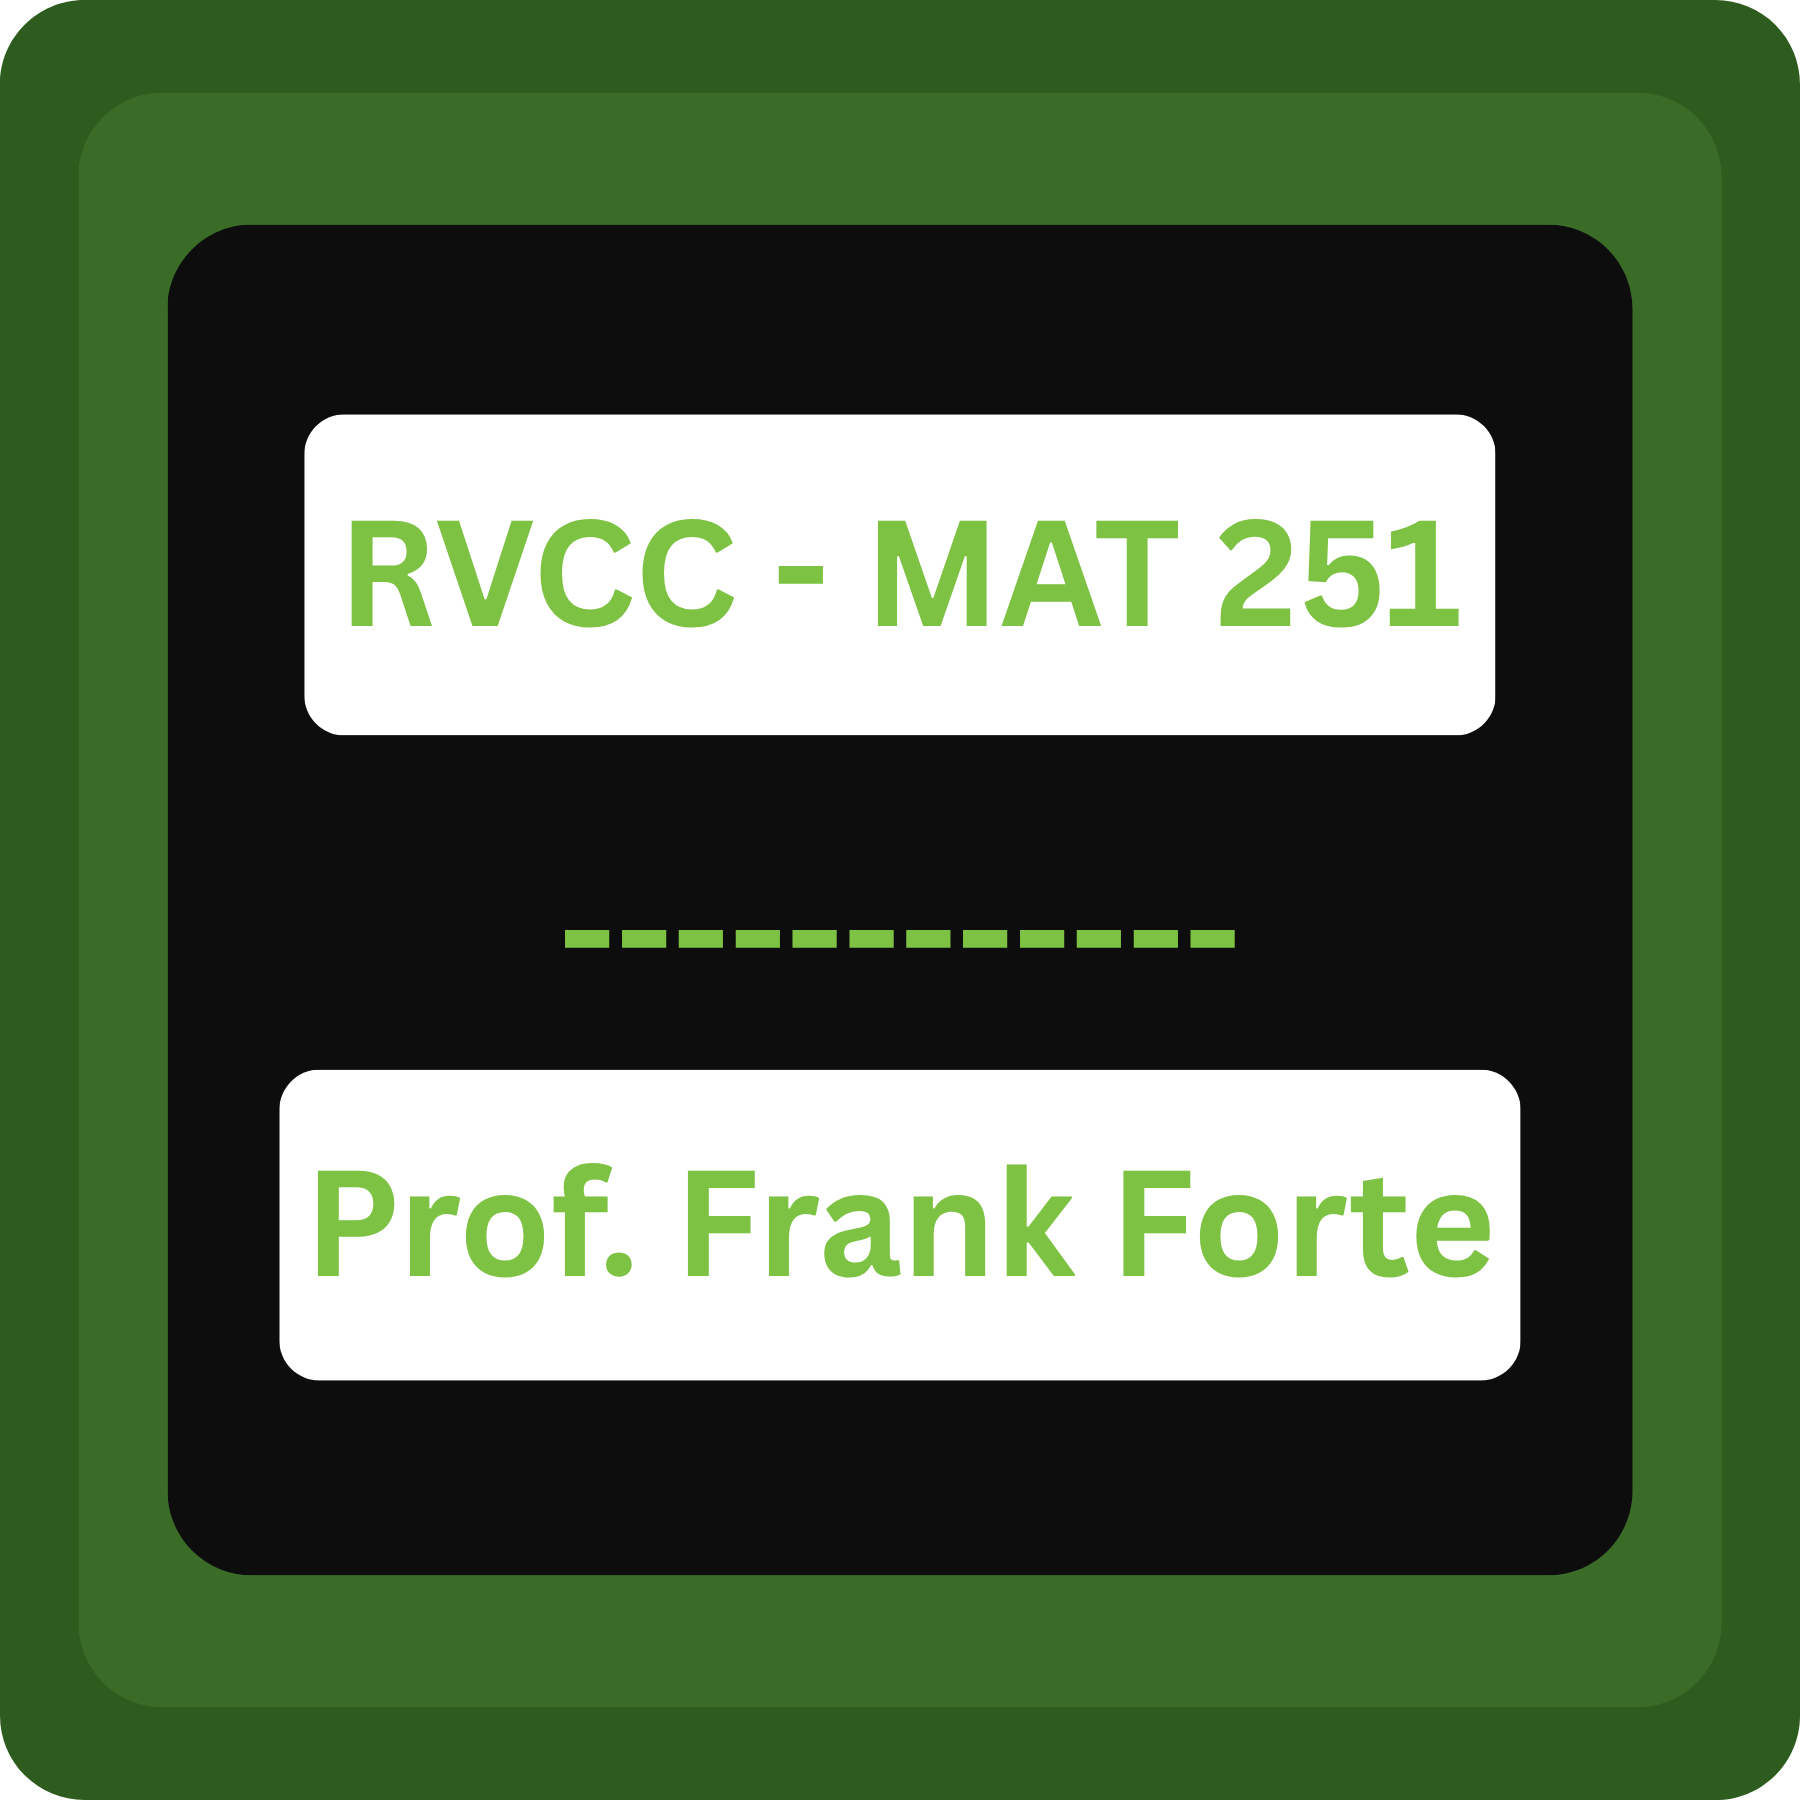
\includegraphics[width=0.9\linewidth]{RVCC - MAT 251.png}
    \caption{Caption}
    \label{fig:placeholder}
\end{figure}

\newpage

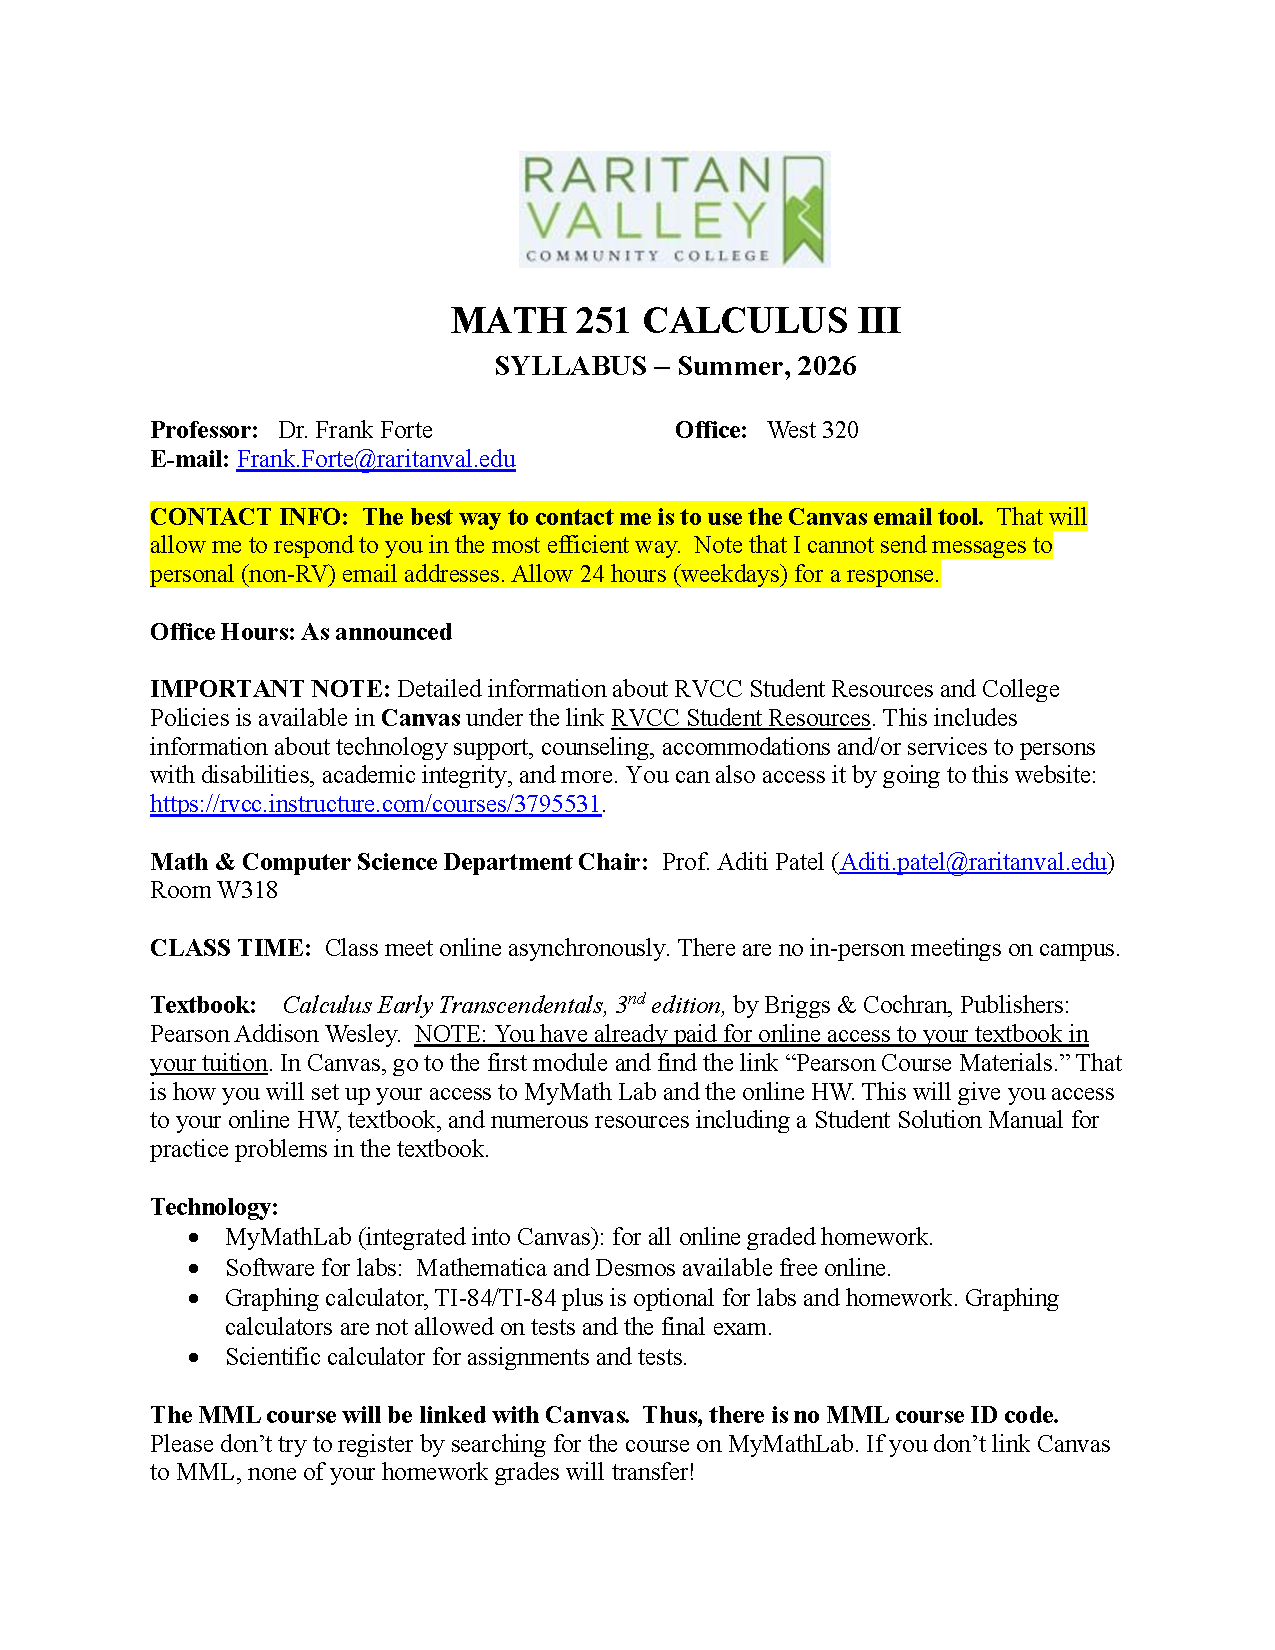
\includepdf[pages=-]{Syllabus Calculus 3 SU26 OL Forte.pdf} 

\newpage

\tableofcontents

\newpage
\section{Resources:}
\begin{itemize}
    \item Calculus I and II Review: \href{https://www.khanacademy.org/math/ap-calculus-bc}{Khan Academy} \cite{collegeboard_apcalcbc, khanacademy_calcbc}
    \item Professor Forte: \href{https://www.youtube.com/watch?v=NJiaIr5Y2VU&list=PLVOT1I6lLvjfDhACPSMXam2diM0IBR3hl}{Youtube} \cite{forte_calc3_2025}
    \item Paul's Online Math Notes: \href{https://tutorial.math.lamar.edu/Classes/CalcIII/CalcIII.aspx}{Calculus 3} \cite{dawkins_calc3}
\end{itemize}

\section{Unit 13:}
    \subsection{Lesson Plan:}
        \begin{itemize}
            \item \href{https://www.youtube.com/watch?v=NJiaIr5Y2VU&list=PLVOT1I6lLvjfDhACPSMXam2diM0IBR3hl&index=1&t=1s}{Vectors}
            \item \href{https://www.youtube.com/watch?v=OggR4c3UgKg&list=PLVOT1I6lLvjfDhACPSMXam2diM0IBR3hl&index=2}{Cross Products and Dot Products}
            \item \href{https://www.youtube.com/watch?v=-NPH_D1SqJk&list=PLVOT1I6lLvjfDhACPSMXam2diM0IBR3hl&index=3}{Lines and Planes}
        \end{itemize}
    
    \subsection{Labs/Homework/Discussions:}
        \paragraph{Discussion \#1 Introductions:}
            Hi my name is Noah Berns, I’m a rising junior at Morristown High school. I’m interested in pursuing a career in math, I’m an avid reader and fantasy head. I spend my free time playing board games with
friends. I’m taking this course because I’m looking to accelerate my my mathematical career and to explore new and interesting concepts. This isn't my fist time taking an a-synchronous class so my advice would be to pace yourself, all of the work you need to do can seem daunting and taking it in chunks both helps with stress and comprehension.
            
        \paragraph{Lab 0 - Introduction to Mathematica (not collected):}
            \input{Unit 13/Lab 0 - Introduction to Mathematica (not collected)}
            
        \paragraph{Homework 13.1 - 13.3:}
            \input{Unit 13/Homework 13.1 - 13.3}
            
        \paragraph{Discussion \#2 Vectors and Dot Products:}
            \begin{itemize}
    \item A vector is something that represents both magnitude and direction.
    \item  Arithmetically you can add three vectors by adding their respective components: $\vec{v} + \vec{u} + \vec{w} = \langle v_1 + u_1 + w_1, v_2 + u_2 + w_2, v_3 + u_3 + w_3 \rangle$. However visually you would connect each vector head to tail and apply the triangle rule to find the resultant. 
    \item To subtract two vectors arithmetically you subtract the respective components: $\vec{v} - \vec{u} = \langle v_1 - u_1, v_2 - u_2, v_3 - u_3 \rangle$. However visually you would flip the direction of the vector $\vec{u}$ and connect them head to tail and apply the triangle rule.
    \item A scalar is a measure of a physical quantity determined solely by it's magnitude. The dot product is the work done by a force and distance vector as we'll as the angle between to vectors.
\end{itemize}

            
        \paragraph{Lab 1 - (Sec. 13.1 - 13.5):}
            \begin{sleekbox}[palTeal]{Problem #1}
    \begin{question}\leavevmode\par\medskip
        \anglevector{1,3,5}+\anglevector{7,-2,-4}
    \end{question}\leavevmode\par\medskip
    
    \begin{solution}\leavevmode\par\medskip
        \anglevector{1+7,3-2,5-4} = \anglevector{8,1,1}
    \end{solution}
\end{sleekbox}

\begin{sleekbox}[palTeal]{Problem #2}
    \begin{question}\leavevmode\par\medskip
        \anglevector{1,3,5} - \anglevector{7,-2,-4}
    \end{question}\leavevmode\par\medskip
        
    \begin{solution}\leavevmode\par\medskip
        \anglevector{-6,5,9}
    \end{solution}
\end{sleekbox}

\begin{sleekbox}[palTeal]{Problem #3}
    \begin{question}\leavevmode\par\medskip
        6\anglevector{1,3,5}
    \end{question}\leavevmode\par\medskip
        \anglevector{6,18,30}
    \begin{solution}\leavevmode\par\medskip
        
    \end{solution}
\end{sleekbox}

\begin{sleekbox}[palTeal]{Problem #4}
    \begin{question}\leavevmode\par\medskip
        \anglevector{1,3,5} \cdot \anglevector{7,-2,-4}
    \end{question}\leavevmode\par\medskip

    \begin{solution}\leavevmode\par\medskip
        $7-6-20=-19$
    \end{solution}
\end{sleekbox}


\begin{sleekbox}[palTeal]{Problem #5}
    \begin{question}\leavevmode\par\medskip
        \norm{\anglevector{1,3,5}}
    \end{question}\leavevmode\par\medskip

    \begin{solution}\leavevmode\par\medskip
        \sqrt{1+9+25} = \sqrt{35}
    \end{solution}
\end{sleekbox}

\begin{sleekbox}[palTeal]{Problem #6}
    \begin{question}\leavevmode\par\medskip
        \norm{\anglevector{7,-2,-4}}
    \end{question}\leavevmode\par\medskip
    
    \begin{solution}\leavevmode\par\medskip
        \sqrt{49+4+16} = \sqrt{69}
    \end{solution}
\end{sleekbox}

\begin{sleekbox}[palTeal]{Problem #7}
    \begin{question}\leavevmode\par\medskip
        Find the angle between \anglevector{1,3,5} and \anglevector{7,-2,-4}.
    \end{question}\leavevmode\par\medskip

    \begin{solution}\leavevmode\par\medskip
        \[
        \anglevector{1,3,5} \cdot \anglevector{7,-2,-4} = \norm{\anglevector{1,3,5}}\norm{\anglevector{7,-2,-4}}\cos(\theta) \implies \frac{-19}{\sqrt{2415}} = \cos(\theta)
        \]
        \[
        \implies \theta =\cos^{-1}(\frac{-19}{\sqrt{2415}}) \approx 1^{\circ}\footnotemark
        \]
    \end{solution}\footnotetext{Rounded to the 5th decimal place.}
\end{sleekbox}

\begin{sleekbox}[palTeal]{Problem #8}
    \begin{question}\leavevmode\par\medskip
        Find the dot product of the vectors \anglevector{7,3,-1,4},\anglevector{5,9,2,5} \in \R^4 .
    \end{question}\leavevmode\par\medskip

    \begin{solution}\leavevmode\par\medskip
        \anglevector{7,3,-1,4} \cdot\anglevector{5,9,2,5} = 35 + 27 - 2 + 20 = 80
    \end{solution}
\end{sleekbox}

\begin{sleekbox}[palTeal]{Problem #9}
    \begin{question}\leavevmode\par\medskip
        Given two vectors whose dot product is zero. What can you say about the
        vectors? Give an example of two vectors with this property.
    \end{question}\leavevmode\par\medskip

    \begin{solution}\leavevmode\par\medskip
        \[
        \forall \, \Vec{u},\Vec{v}\in V_n \subset \R^n , \text{where } \Vec{u} \cdot \Vec{v} = 0 \implies \cos(\theta) = 0 \implies \theta = 0 + 2\pi c, \text{ for } c \in \mathbb{Z}
        \]
        Thus both vectors must be orthogonal to one another. An example of this property are the unit vectors where the dot product for any 2 unique standard vectors $(\hat{i},\hat{j},\hat{k},\dots)$ is zero. Thus all of the standard unit vectors are orthogonal to one another.
    \end{solution}
\end{sleekbox}

\begin{sleekbox}[palTeal]{Problem #10}
    \begin{question}\leavevmode\par\medskip
        \begin{parts}
            \item Find a vector orthogonal to the vectors \anglevector{2,17,5}, and \anglevector{-1,-4,-7}.
            \item Show (by calculations on Mathematica) that these vectors are orthogonal.
            \item Graph the three vectors.
        \end{parts}
        
    \end{question}\leavevmode\par\medskip

    \begin{solution}\leavevmode\par\medskip 
        \begin{parts}
            \item  \[
            \anglevector{2,17,5} \times \anglevector{-1,-4,-7} = \begin{vmatrix} \hat{i} & \hat{j} & \hat{k} \\ 2 & 17 & 5 \\ -1 & -4 & -7 \end{vmatrix} = \begin{vmatrix} 17 & 5 \\ -4 & -7 \end{vmatrix} \hat{i} - \begin{vmatrix} 2 & 5 \\ -1 & -7 \end{vmatrix} \hat{j} = \begin{vmatrix} 2 & 17 \\ -1 & -4\end{vmatrix} \hat{k}
            \]
    
            \[
            = \anglevector{-99,9,9}
            \]

            \item \[
                \anglevector{2,17,5} \cdot \anglevector{-99,9,9} = 0 \wedge \anglevector{-1,-4,-17} \cdot \anglevector{-99,9,9} = 0
            \]
        \end{parts}
       
        
    \end{solution}
\end{sleekbox}

\begin{sleekbox}[palTeal]{Problem #11}
    \begin{question}\leavevmode\par\medskip
    Sketch the surface by hand (if possible) and also using Mathematica (plot3D):
    \begin{parts}
        \item $f(x,y) = 1-x^2-y^2$
        \item $f(x,y)=\sqrt{1-x^2 -z^2}$
    \end{parts}
        
    \end{question}\leavevmode\par\medskip
       
    \begin{solution}\leavevmode\par\medskip
         \begin{figure}[H]
            \centering
            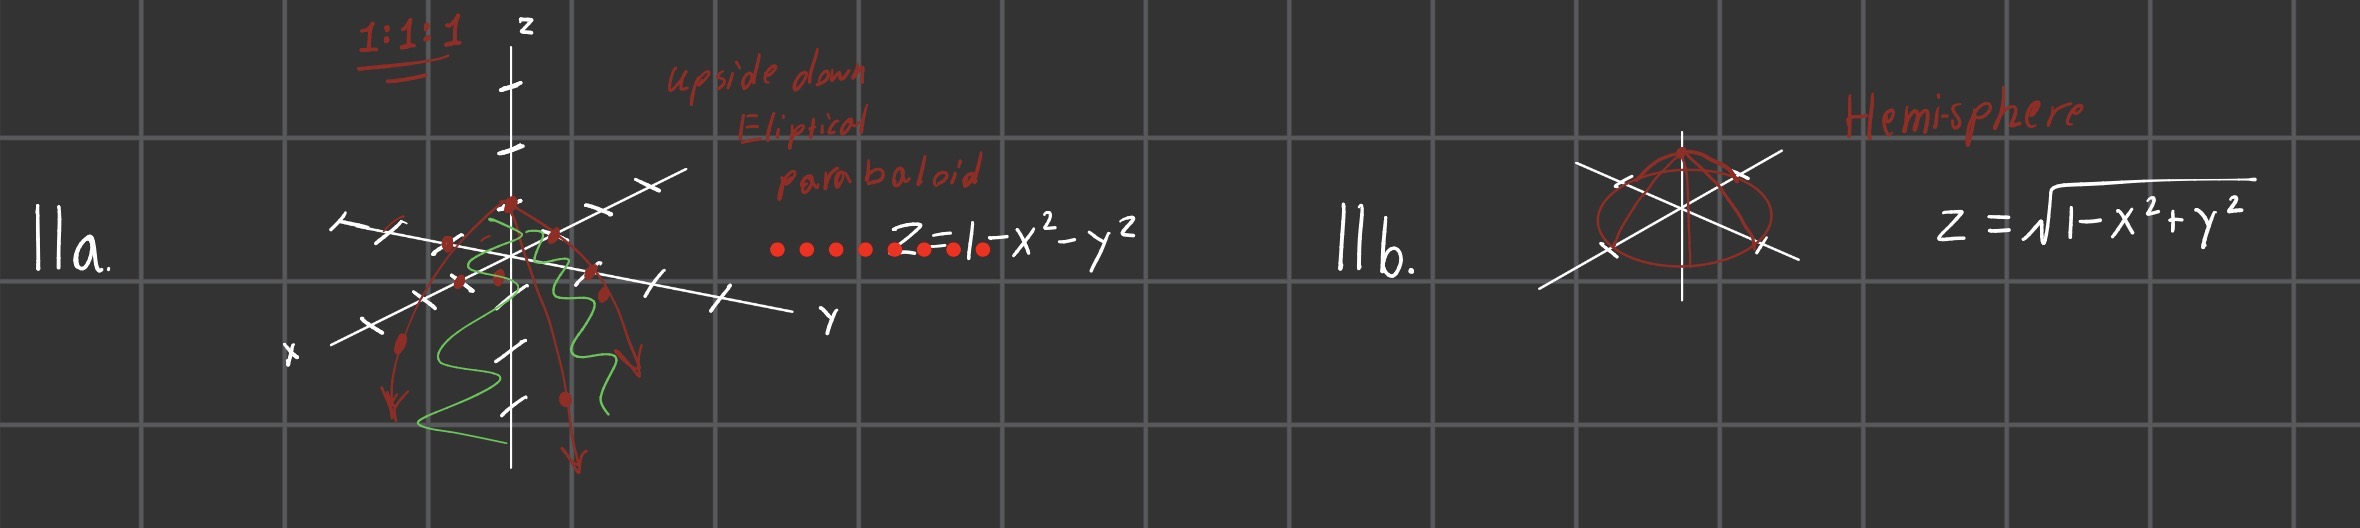
\includegraphics[width=0.75\linewidth]{Unit 13//Lab 1/IMG_2660.jpeg}
            \label{fig:placeholder}
        \end{figure}
    \end{solution}

\end{sleekbox}
            
        \paragraph{Homework 13.4 - 13.6:}
            \input{Unit 13/Homework 13.4 - 13.6}
            
        \paragraph{Discussion \#3 Potato Chips and 3D Surfaces:}
            \begin{enumerate}
    \item The shape of a Pringle is a hyperbolic paraboloid. 
    \item The Procter \& Gamble R\&D department set out to fix the problems with conventional potato chips. Chemist Fredric Baur, was the one to develop the iconic shape spent 2+ years researching the design while Alexander Liepa was the one who perfected the modern day Pringle.
    \item According to the Pringles company the hyperbolic paraboloid is perfect because it solved the problems of the classic potato chip "which were often greasy, stale and broken". Plus the design is extremely space efficient. 
\end{enumerate}

\begin{MLAENV}
    \begin{itemize}
        \item Pringles. (2023). FAQ | Pringles®. Pringles.com 
        
        \url{https://www.pringles.com/en-us/faq.html}
    
        \item Wikipedia Contributors. (2019, April 12). Pringles. Wikipedia; Wikimedia Foundation.
        
        \url{https://en.wikipedia.org/wiki/Pringles}
    \end{itemize}
\end{MLAENV}


\section{Unit 14:}
    \subsection{Lesson Plan:}
        \begin{itemize}
            \item \href{https://www.youtube.com/watch?v=HBRli7Jv_Ng&list=PLVOT1I6lLvjfDhACPSMXam2diM0IBR3hl&index=4}{Vector Valued Functions}
            \item \href{https://www.youtube.com/watch?v=gz-bhgt3NbQ&list=PLVOT1I6lLvjfDhACPSMXam2diM0IBR3hl&index=5}{Length of a Curve}
            \item \href{youtube.com/watch?v=hUq-uHI7Mpw&list=PLVOT1I6lLvjfDhACPSMXam2diM0IBR3hl&index=6}{Curvature and Normal Vectors Pt.1}
            \item \href{https://www.youtube.com/watch?v=eLPrbhmgC0g&list=PLVOT1I6lLvjfDhACPSMXam2diM0IBR3hl&index=7a}{Binormal Vectors and Torsion Pt.2}
        \end{itemize}
    
    \subsection{Labs/Homework/Discussions:}
        \paragraph{Homework 14.1 - 14.2:}
            \input{Unit 14/Homework 14.1 - 14.2}
            
        \paragraph{Lab 2 - Chapter 14:}
            \setcounter{qcount}{0}

\begin{sleekbox}[palCoral]{Problem \#1}
    \begin{question}\leavevmode\par\medskip
       Find the angle between the vectors $\anglevector{2, 4, 6}$ and $\anglevector{1, 5, 4}$. Show work by hand and your verification on Mathematica.
    \end{question}\leavevmode\par\medskip
    \begin{solution}\leavevmode\par\medskip
    
    \end{solution}
    
\end{sleekbox}

\begin{sleekbox}[palCoral]{Problem \#2}
    \begin{question}\leavevmode\par\medskip
       Find the work done by the force $\Vec{F} = \anglevector{3, 1, 7}$; the object displaced by the force
undergoes a displacement $\Vec{d} = \anglevector{5, 3, 2}$.
    \end{question}\leavevmode\par\medskip
    \begin{solution}\leavevmode\par\medskip
    
    \end{solution}
    
\end{sleekbox}

\begin{sleekbox}[palCoral]{Problem \#3}
    \begin{question}\leavevmode\par\medskip
       Find the force on an electron $\left(charge = q = 1.6 * 10^{-19} Coulombs\right)$ that is moving
    along the y axis with a speed of $8\times10^6 m/sec$ as it enters a magnetic field of strength 1.1
    tesla, directed in the positive z direction. (See example 6, page 841, section 13.4, for a
    similar problem in your book.)
    \end{question}\leavevmode\par\medskip
    \begin{solution}\leavevmode\par\medskip
    
    \end{solution}
    
\end{sleekbox}

\begin{sleekbox}[palCoral]{Problem \#4}
    \begin{question}\leavevmode\par\medskip
       Sketch the \textit{helix}: $\Vec{r}(t) = \anglevector{\cos(t), \sin(t),t}$
    \end{question}\leavevmode\par\medskip
    \begin{solution}\leavevmode\par\medskip
    
    \end{solution}
    
\end{sleekbox}

\begin{sleekbox}[palCoral]{Problem \#5}
    \begin{question}\leavevmode\par\medskip
       Write the parametric equations of a line that goes through the origin and is parallel to
    the vector $\anglevector{2, 4, 6}$. Then write the vector expression for the same line.
    \end{question}\leavevmode\par\medskip
    \begin{solution}\leavevmode\par\medskip
    
    \end{solution}
    
\end{sleekbox}

\begin{sleekbox}[palCoral]{Problem \#6}
    \begin{question}\leavevmode\par\medskip
       Write a vector expression for the curve which is given by $y=x \text{ and } z=x^2 + y^2$ using the parameter $t$. Then graph it on Mathematica.
    \end{question}\leavevmode\par\medskip
    \begin{solution}\leavevmode\par\medskip
    
    \end{solution}
    
\end{sleekbox}

\begin{sleekbox}[palCoral]{Problem \#7}
    \begin{question}\leavevmode\par\medskip
    For the function y = f(x), assuming f(x) is twice differentiable, this is another formula
    for curvature:
    \[
    k(x) = \frac{|f''(x)|}{\left( 1 + f'(x)^2 \right)^\frac{3}{2}}
    \]
        \begin{parts}
            \item Find the curvature for $f(x) = \ln(x), (x > 0)$ and find the point at which it is a maximum.
            \item What is the value of the maximum curvature?
            \item Find the curvature for $f(x) = e^x$ and find the point at which it is a maximum.
            \item What is the value of the maximum curvature?
            \item Compare your answers to parts b and d. What are the results? Why might this be happening?
        \end{parts}
    \end{question}\leavevmode\par\medskip
    \begin{solution}\leavevmode\par\medskip
        \begin{parts}
            \item 
            \item 
            \item 
            \item 
            \item 
            \item 
        \end{parts}
    \end{solution}
    
\end{sleekbox}

\newpage


        \paragraph{Homework 14.3 - 14.5:}
            \input{Unit 14/Homework 14.3 - 14.5}

\section{Chapter 13 \& 14 Test:}

\section{Unit 15:}
    \subsection{Lesson Plan:}
        \begin{itemize}
            \item \href{https://www.youtube.com/watch?v=jcgdm4dNoG0&list=PLVOT1I6lLvjfDhACPSMXam2diM0IBR3hl&index=8}{Level Curves}
            \item \href{https://www.youtube.com/watch?v=jcgdm4dNoG0&list=PLVOT1I6lLvjfDhACPSMXam2diM0IBR3hl&index=8}{Limits and Continuity}
            \item \href{https://www.youtube.com/watch?v=Lk0N24reXEk&list=PLVOT1I6lLvjfDhACPSMXam2diM0IBR3hl&index=10}{Partial Derivatives}
            \item \href{https://www.youtube.com/watch?v=yyJyuHEkPZ8&list=PLVOT1I6lLvjfDhACPSMXam2diM0IBR3hl&index=11}{Chain Rule}
            \item \href{https://www.youtube.com/watch?v=frE1UFRhflg&list=PLVOT1I6lLvjfDhACPSMXam2diM0IBR3hl&index=12}{Directional Derivatives and the Gradient Pt.1}
            \item \href{https://www.youtube.com/watch?v=nI_KvqSWHjo&list=PLVOT1I6lLvjfDhACPSMXam2diM0IBR3hl&index=13}{Directional Derivatives and the Gradient Pt.2}
            \item \href{https://www.youtube.com/watch?v=zrzbNsK3C8I&list=PLVOT1I6lLvjfDhACPSMXam2diM0IBR3hl&index=14}{Tangent Planes and Linear Approximations}
            \item \href{https://www.youtube.com/watch?v=Sfb5eUoG4Q0&list=PLVOT1I6lLvjfDhACPSMXam2diM0IBR3hl&index=15}{Extrema Pt.1}
            \item \href{https://www.youtube.com/watch?v=LSp-1lQ0lHI&list=PLVOT1I6lLvjfDhACPSMXam2diM0IBR3hl&index=16}{Extrema Pt.2}
            \item \href{https://www.youtube.com/watch?v=aAgkhoaggSM&list=PLVOT1I6lLvjfDhACPSMXam2diM0IBR3hl&index=17}{Extrema Pt.3}
            \item \href{https://www.youtube.com/watch?v=R2rQdQkG-i8&list=PLVOT1I6lLvjfDhACPSMXam2diM0IBR3hl&index=18}{LaGrange Multipliers Pt.1}
            \item \href{https://www.youtube.com/watch?v=XQlKolWjr14&list=PLVOT1I6lLvjfDhACPSMXam2diM0IBR3hl&index=19}{LaGrange Multipliers Pt.2}
        \end{itemize}
    
    \subsection{Labs/Homework/Discussions:}
        \paragraph{Homework 15.1 - 15.2:}
            \input{Unit 15/Homework 15.1 - 15.2}

        \paragraph{Discussion \#4 Partial Derivatives:}
            \input{Unit 15/Discussion #4 Partial Derivatives}

        \paragraph{Homework 15.3 - 15.4:}
            \input{Unit 15/Homework 15.3 - 15.4}

        \paragraph{Lab 3 - (Sec. 15.1 - 15.3):}
            \input{Unit 15/Lab 3 - (Sec. 15.1 - 15.3)}

        \paragraph{Lab 4 - (Ch. 15 Part 2):}
            \input{Unit 15/Lab 4 - (Ch. 15 Part 2)}

        \paragraph{Homework 15.5 - 15.6:}
            \input{Unit 15/Homework 15.5 - 15.6}

        \paragraph{Discussion \#5 Hessian Matrix (Sec. 15.7):}
            \input{Unit 15/Discussion #5 Hessian Matrix (Sec. 15.7)}

        \paragraph{Homework 15.7 - 15.8:}
            \input{Unit 15/Homework 15.7 - 15.8}

        \paragraph{Lab 5 - (Ch.15 Part 3):}
            \input{Unit 15/Lab 5 - (Ch.15 Part 3)}

\section{Chapter 15 Test:}

\section{Unit 16:}
    \subsection{Lesson Plan:}
        \begin{itemize}
            \item \href{https://www.youtube.com/watch?v=Ytj-Gbl1KDY&list=PLVOT1I6lLvjfDhACPSMXam2diM0IBR3hl&index=20}{Double Integrals Over Rectangular Regions}
            \item \href{https://www.youtube.com/watch?v=xrHwl5r1rJA&list=PLVOT1I6lLvjfDhACPSMXam2diM0IBR3hl&index=21}{Double Integrals Over General Regions}
            \item \href{https://www.youtube.com/watch?v=-IMve2eGg9I&list=PLVOT1I6lLvjfDhACPSMXam2diM0IBR3hl&index=22}{Double Integrals Over Polar Regions}
            \item \href{https://www.youtube.com/watch?v=jNyhF-AjWFw&list=PLVOT1I6lLvjfDhACPSMXam2diM0IBR3hl&index=23}{Triple Integrals}
            \item \href{https://www.youtube.com/watch?v=sWEyTlzSY3E&list=PLVOT1I6lLvjfDhACPSMXam2diM0IBR3hl&index=24}{Cylindrical Coordinates and Triple Integrals}
            \item \href{https://www.youtube.com/watch?v=BbL3nfgm-as&list=PLVOT1I6lLvjfDhACPSMXam2diM0IBR3hl&index=25}{Spherical Coordinates and Triple Integrals}
            \item \href{https://www.youtube.com/watch?v=wZcT1D2x4bs&list=PLVOT1I6lLvjfDhACPSMXam2diM0IBR3hl&index=26}{Center of Mass and Density Pt.1}
            \item \href{http://youtube.com/watch?v=k_FCcJ51S0c&list=PLVOT1I6lLvjfDhACPSMXam2diM0IBR3hl&index=27}{Center of Mass and Density Pt.2}
            \item \href{https://www.youtube.com/watch?v=lp-ZTiy1_sw&list=PLVOT1I6lLvjfDhACPSMXam2diM0IBR3hl&index=28}{Introduction to Change of Variables}
            \item \href{https://www.youtube.com/watch?v=WMAPaIM2xIA&list=PLVOT1I6lLvjfDhACPSMXam2diM0IBR3hl&index=29}{Jacobians and Change of Variables}
            \item \href{https://www.youtube.com/watch?v=s2dLHMnRpms&list=PLVOT1I6lLvjfDhACPSMXam2diM0IBR3hl&index=30}{Jacobians for Three Variables}
        \end{itemize}
    
    \subsection{Labs/Homework/Discussions:}
        \paragraph{Homework 16.1 - 16.2:}
            \input{Unit 16/Homework 16.1 - 16.2}

        \paragraph{Discussion \#6 Double Integrals:}
            \input{Unit 16/Discussion #6 Double Integrals}

        \paragraph{Lab 6 - (Ch.16 Part 1):}
            \input{Unit 16/Lab 6 - (Ch.16 Part 1)}

        \paragraph{Homework 16.3 - 16.5:}
            \input{Unit 16/Homework 16.3 - 16.5}

        \paragraph{Discussion \#7 Spherical Coordinates and the Jacobian:}
            \input{Unit 16/Discussion #7 Spherical Coordinates and the Jacobian}

        \paragraph{Homework 16.6 - 16.7:}
            \input{Unit 16/Homework 16.6 - 16.7}

        \paragraph{Lab 7 - (Ch.16 Part 2):}
            \input{Unit 16/Lab 7 - (Ch.16 Part 2)}

\section{Chapter 16 Test:}

\section{Unit 17:}
    \subsection{Lesson Plan:}
        \begin{itemize}
            \item \href{https://www.youtube.com/watch?v=qD6xUP-1-DY&list=PLVOT1I6lLvjfDhACPSMXam2diM0IBR3hl&index=31}{Vector Fields}
            \item \href{https://www.youtube.com/watch?v=sUYdWoHrI2g&list=PLVOT1I6lLvjfDhACPSMXam2diM0IBR3hl&index=32}{Line Integrals Pt.1}
            \item \href{https://www.youtube.com/watch?v=mJoq7zZWGoA&list=PLVOT1I6lLvjfDhACPSMXam2diM0IBR3hl&index=33}{Line Integrals Pt.2 (Circulation and Flux)}
            \item \href{https://www.youtube.com/watch?v=aovijT468Mc&list=PLVOT1I6lLvjfDhACPSMXam2diM0IBR3hl&index=34}{Conservative Vector Fields}
            \item \href{https://www.youtube.com/watch?v=cXIXR8sEJaA&list=PLVOT1I6lLvjfDhACPSMXam2diM0IBR3hl&index=35}{Green's Theorem Pt.1}
            \item \href{https://www.youtube.com/watch?v=z2-6KgQEjH8&list=PLVOT1I6lLvjfDhACPSMXam2diM0IBR3hl&index=36}{Green's Theorem Pt.2 (Flux)}
            \item \href{https://www.youtube.com/watch?v=n0bVPtiJ2nE&list=PLVOT1I6lLvjfDhACPSMXam2diM0IBR3hl&index=37}{Divergence and Curl}
            \item \href{https://www.youtube.com/watch?v=GbFP_fLCu7w&list=PLVOT1I6lLvjfDhACPSMXam2diM0IBR3hl&index=38}{Surface Integrals}
            \item \href{https://www.youtube.com/watch?v=55ibSTgi7AY&list=PLVOT1I6lLvjfDhACPSMXam2diM0IBR3hl&index=41}{Stokes' Theorem}
            \item \href{https://www.youtube.com/watch?v=2l9DUwTx9hE&list=PLVOT1I6lLvjfDhACPSMXam2diM0IBR3hl&index=39}{Divergence Theorem}
        \end{itemize}
    
    \subsection{Labs/Homework/Discussions:}
        \paragraph{Homework 17.1 - 17.2:}
            \input{Unit 17/Homework 17.1 - 17.2}

        \paragraph{Discussion \#8 Vector Fields and Line Integrals:}
            \input{Unit 17/Discussion #8 Vector Fields and Line Integrals}

        \paragraph{Homework 17.3 - 17.4:}
            \input{Unit 17/Homework 17.3 - 17.4}

        \paragraph{Lab 8 - Chapter 17:}
            \input{Unit 17/Lab 8 - Chapter 17}

        \paragraph{Homework 17.5 - 17.8:}
            \input{Unit 17/Homework 17.5 - 17.8}

\section{Final Exam:}

\end{document}